
\documentclass[11pt, twocolumn]{IEEEtran}
\usepackage{amsmath}
\usepackage{amsfonts}
\usepackage{mathrsfs}
\usepackage{lscape}
\usepackage{listings}
\usepackage{graphicx} % Allows for importing of figures
\usepackage{color} % Allows for fonts to be colored
\usepackage{comment} % Allows for comments to be made
\usepackage{accents} % Allows for accents to be made above and below text
%\usepackage{undertilde} % Allows for under tildes to take place for vectors and tensors
\usepackage[table]{xcolor}
\usepackage{array,ragged2e}
\usepackage{hyperref}
\usepackage{framed} % Allows boxes to encase equations and such
\usepackage{subcaption} % Allows for figures to be side-by-side
\usepackage{float} % Allows for images to not float in the document
\usepackage{booktabs}
%\usepackage[margin=0.75in]{geometry}
\usepackage[final]{pdfpages}
\usepackage{enumitem}
\usepackage[section]{placeins}
\usepackage{cite}
%%%%%%%%%%%%%%%%%%%%%%%%%  Function used to generate vectors and tensors %%%%%%%%%
\usepackage{stackengine}
\stackMath
\newcommand\tensor[2][1]{%
	\def\useanchorwidth{T}%
	\ifnum#1>1%
	\stackunder[0pt]{\tensor[\numexpr#1-1\relax]{#2}}{\scriptscriptstyle \sim}%
	\else%
	\stackunder[1pt]{#2}{\scriptscriptstyle \sim}%
	\fi%
}
%%%%%%%%%%%%%%%%%%%

\definecolor{mygrey}{rgb}{0.97,0.98,0.99}
\definecolor{codeblue}{rgb}{.2,0,1}
\definecolor{codered}{rgb}{1,0,0}
\definecolor{codegreen}{rgb}{0.3,0.33,0.12}
\definecolor{codegray}{rgb}{0.5,0.5,0.5}
\definecolor{codepurple}{rgb}{0.55,0.0,0.55}
\definecolor{codecyan}{rgb}{0.0,.4,.4}

\lstdefinestyle{mystyle}{
	backgroundcolor=\color{mygrey},   
	commentstyle=\color{codegreen},
	keywordstyle=\color{codeblue},
	stringstyle=\color{codepurple},
	numberstyle=\tiny\color{codegray},
	basicstyle=\footnotesize,
	breakatwhitespace=false,         
	breaklines=true,                 
	captionpos=b,                    
	keepspaces=true, 
	numbers=left,                    
	numbersep=5pt,                  
	showspaces=false,                
	showstringspaces=false,
	showtabs=false,                  
	tabsize=2
}
\lstset{style=mystyle}

\lstset{language=Matlab,backgroundcolor=\color{mygrey}}
\usepackage{lastpage}
\usepackage{fancyhdr}
\pagestyle{fancy}
%%%\lhead{\large{Nik Benko, Peter Creveling}} 
%\chead{\large{\textbf{Automatic Segmentation of Micro CT Images \\  \normalsize{ME EN 6035 Final Project} \\ \small{Nik Benko, Peter Creveling}}}}
%\rhead{\today}
\cfoot{[\thepage\ of \pageref{LastPage}]}
\fancyheadoffset{.5cm}
\setlength{\parindent}{0cm}
\usepackage[left=.75in, right=0.750in, top=1.00in,bottom=1.00in]{geometry}
\usepackage{microtype} 
\usepackage{setspace}
%\doublespace
%%%%%%%%%%%%%%%%%%%%%%%%%%%%%%%%%%%%%%%%%%%%%%%%%%%%%%%%%%%%%%%%%%%%%%%%%%
% git testing ii

\begin{document}
\title{ Statistical Validation of a Novel Porosity Segmentation Algorithm With X-ray Micro-computed Tomography of Ceramic Matrix Composites  \\ \bigskip \normalsize{ME EN 6035 Final Project}}
\author{Nikolaus Benko and Peter Creveling}
\maketitle


\begin{abstract} 
In this study, the accuracy of automatic segmentation methods were statistically compared to a manual segmentation method. Segmentation was performed on X-ray Micro-computed Tomography images of fiber-reinforced ceramic matrix composites in order to extract porosity from the surrounding microscturcture. Four different automatic segmentation methods were investigated. Statistical analysis techniques including one-way and two-way ANOVA, multiple comparisons, and 2 by 2 factorial were performed to determine how the methods compared. It was found that using a combination of pre-segmentation filtering, 3-D machine learning segmentation, and post-process edge erosion had the best agreement with manual segmentation.
\end{abstract}

\text{Keywords:}
\textbf{X-ray Micro-computed Tomography, Ceramic Matrix Composites, Image Segmentation, ANOVA, Tukey's HSD, Factorial Analysis}

\section{Introduction and Background}

Fiber-reinforced ceramic matrix composites (CMCs) are widely used in the aerospace industry due to their high specific strength, high stiffness, and their ability to withstand prolonged exposure to extreme high-temperature and oxidative environments. Despite their increased use, the physics governing their manufacturing, stochastic microstructure, and long-term structural performance remains an active area of research. Understanding the complete life-cycle of CMCs is critical towards improving  existing and future applications of CMCs. In recent years, the emerging practice of in situ X-ray micro-computed tomography (X-ray $\mu$CT) experiments has proven useful for providing a holistic understanding of the behavior of CMCs on multiple length scales \cite{Larson,Bale,Bale2,Cox,Haboub,Marshall}.\\
Unique to X-ray $\mu$CT is the ability to take through-thickness images of specimens in 3-D. This provides much more information compared to other 2-D surface based techniques. However, processing these images to extract information comes at high computational costs. One of the most common imaging processing operations is segmentation, in which pixels are categorized into two or more groups that correspond to some physical characteristic of the material being imaged. For example, CMC images are often segmented to distinguish between fibers and the surrounding matrix. There exist active areas of research in improving best practices for the segmentation of X-ray $\mu$CT reconstructions. Segmentation techniques vary widely depending on image properties such as noise characteristics, contrast between segments, and edge sharpness. X-ray $\mu$CT of large specimens on the order of tens of millimeters results in an image with a significant signal to noise ratio, making automatic segmentation challenging. Researchers have largely relied on manual segmentation, in which a user classifies each pixel by hand. While accurate, this method is very time consuming and impractical for processing of large data sets as well as being difficult to reproduce. For this reason the development of an automated method of segmentation is desired.\\
In this study, several automatic segmentation strategies were constructed and tested against a manually segmented data sets to determine accuracy. Cross-sections of a 3-D X-ray $\mu$CT image data set were segmented to calculate the porosity of each slice. Porosity was defined as the number of pixels representing materials other than carbon fibers or the surrounding matrix, divided by the total number of pixels in the image. A statistical validation was performed to compare the differences in segmentation ability between the automatic methods and the manual segmentation method.

\section{Materials and Methods}

\subsection{Composite CMC and X-ray $\mu$CT}
This study is an extension of current research being performed in the Utah Composites lab where X-ray $\mu$CT is being utilized to image the entire multi-step manufacturing process of CMCs combined with \textit{in situ} testing in extreme environments. The ultimate goal is to fully quantify the changes of the CMC microstructure throughout their entire life-cycle via methods of segmentation. Iteratively imaging the microstructure over time will provide unprecedented insight to the understanding of these complex materials. To this end, the composite system used consisted of a 8HS satin weave CG Nicalon-fiber fabric infiltrated with SMP-10 matrix. Imaging was performed using a Zeiss Versa-520 X-ray $\mu$CT 3D microscope at the Air Force Research Laboratory (Dayton, OH). In this study, images were analyzed from the pyrolysis step of the manufacturing process after which the resin was cured at 1000$^{\circ}$C.

\subsection{Data}
Images were collected with a scan time of 37.3 hours about a selected region of interest from the center of the entire CMC specimen with approximate dimensions of 60$\times$30$\times$1.5 mm. There were 1980 8-bit images collected with a spatial resolution of 1.21 $\mu$m/voxel. In total, the entire image stack consisted of 22.1GB of information. For this study, a small sub-volume of 500$\times$500$\times$500 pixels was analyzed. Within this sub-volume, both manual and automatic segmentation were performed in order to extract porosity (e.g. cracks or voids) from the surrounding microstructure (e.g. fibers or matrix). It was assumed that the manual segmentation method for porosity calculation was the ``ground truth." The accuracy of the automatic segmentation methods was compared to these results.

\subsection{Automatic Segmentation Methods}
The automatic segmentation methods began with a pre-processing step using a non-local-means filter \cite{buades2011non}. This was performed to remove an optimal amount of noise, induced by the combination of imaging method used and large specimen geometry, while maintaining image fidelity of the material microstructure. Next, a machine learning algorithm known as WEKA segmentation was implemented to perform a binary classification of individual pixels corresponding to either structural materials or pores. This algorithm utilizes a combination of data mining, clustering, classification, regression, visualization, association rules, and feature selection to perform the desired segmentation \cite{Weka}. WEKA can be utilized on both 2-D discrete images as well as 3-D image stacks. Both 2-D and 3-D techniques were executed on the filtered data. From preliminary results as described later in section \ref{RandD}, a method known as Edge Erosion was implemented to further improve agreement between automatic segmentation results and manual segmentation by compensating for the over-prediction of pore edges. In total, there were four automatic segmentation methods executed, 2-D and 3-D WEKA segmentation of the filtered image stacks as well as 2-D and 3-D WEKA segmentation plus Edge Erosion of the filtered image stacks.

\subsection{Statistical Analysis} 
Several different statistical techniques were used to evaluate the segmentation algorithms. First a one-way ANOVA was conducted on the porosity measurements for each technique to determine whether or not automatic calculations of porosity were significantly different from manual calculations. Normality and homoscedasticity were checked by plotting histograms and box plots of the data. Here the null hypothesis is that all methods result in the same mean porosity measurement for the image set. The alternative hypothesis is that some means are not equal. A multiple comparisons analysis (Tukey's HSD) was then conducted to test multiple alternative hypothesis and determine which methods, if any, were statistically different.\\

An additional data set was constructed by calculating the percent error between each of the automatically segmented results and the manually segmented results. This data was no longer dependent on the underlying image and could be treated as a random variable. Normality of data was checked by plotting the histograms for each automatic method. Finally, the four automatic segmentation methods  were broken into two categories based on algorithm features with ``high" and ``low" treatments for each category. A 2 by 2 factorial and a 2-way ANOVA were performed to determine which algorithm features, Analysis Dimensions (i.e. 2-D versus 3-D WEKA segmentation) and Edge Erosion (i.e. with or without applying edge erosion), most effected the results. A confidence level of 95\% was used for all analyses.\\
In short, the analysis presented provides statistical information on the accuracy of the four automatic segmentation methods compared to manual segmentation. Additionally, this analysis provides insight towards which method has the largest effect on achieving accurate segmentation.

\section{Results and Discussion} \label{RandD}
Histograms of the porosity calculations are shown in Figure \ref{fig:DataHist}. The histograms reveal that most data sets do not meet the condition of normality and contain a heavy left skew. Figure \ref{fig:Boxy} shows the distribution of the data for each segmentation method. This is in fact not surprising as the porosity measurement is based on image content, which is not a random variable. However, variance was approximately equal between data sets suggesting that an ANOVA was still appropriate. From Figure \ref{fig:Boxy}, outliers of porosity segmentation are highlighted in Figure \ref{fig:Outy}. The outliers are largely contributed to image slices between approximately 90 and 115. Interesting though is that this divergence in porosity segmentation is consistent between all automatic algorithms. Mean porosity and standard deviation (STD) are listed in Table \ref{tab:DataTable}. Results from the one-way ANOVA (Table \ref{tab:OneWay}) and multiple comparisons test (Table \ref{tab:mult}) show that there are significant differences ($p<$0.05) in the means of all of the methods except between the manual segmentation and 3-D algorithm with Edge Erosion correction. Specifically the null hypothesis that 3-D with Edge Erosion produces the same results when compared to manual segmentation ($p$=0.081) cannot be rejected.

\begin{figure}[h!]
	\centering
	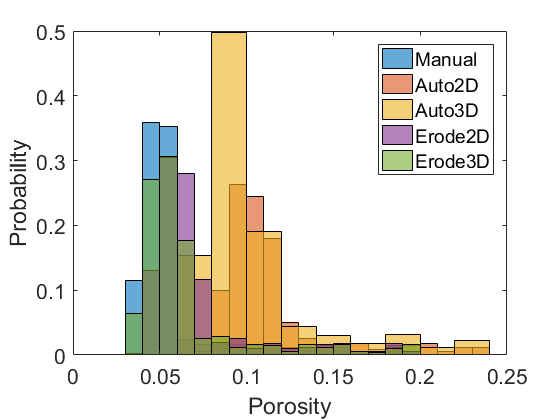
\includegraphics[width=0.5\textwidth]{DataHistograms.png}
	\caption{Histogram of porosity distribution for each segmentation method}
	\label{fig:DataHist}
\end{figure}

\begin{figure}[h!]
	\centering
	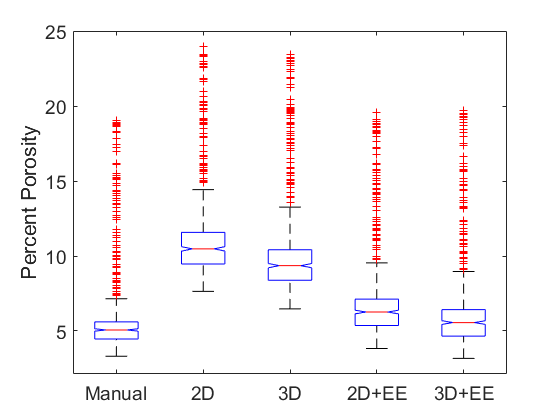
\includegraphics[width=0.5\textwidth]{SuperBoxy.png}
	\caption{Box plots of porosity segmentation for each method.}
	\label{fig:Boxy}
\end{figure}

\begin{figure}[h!]
	\centering
	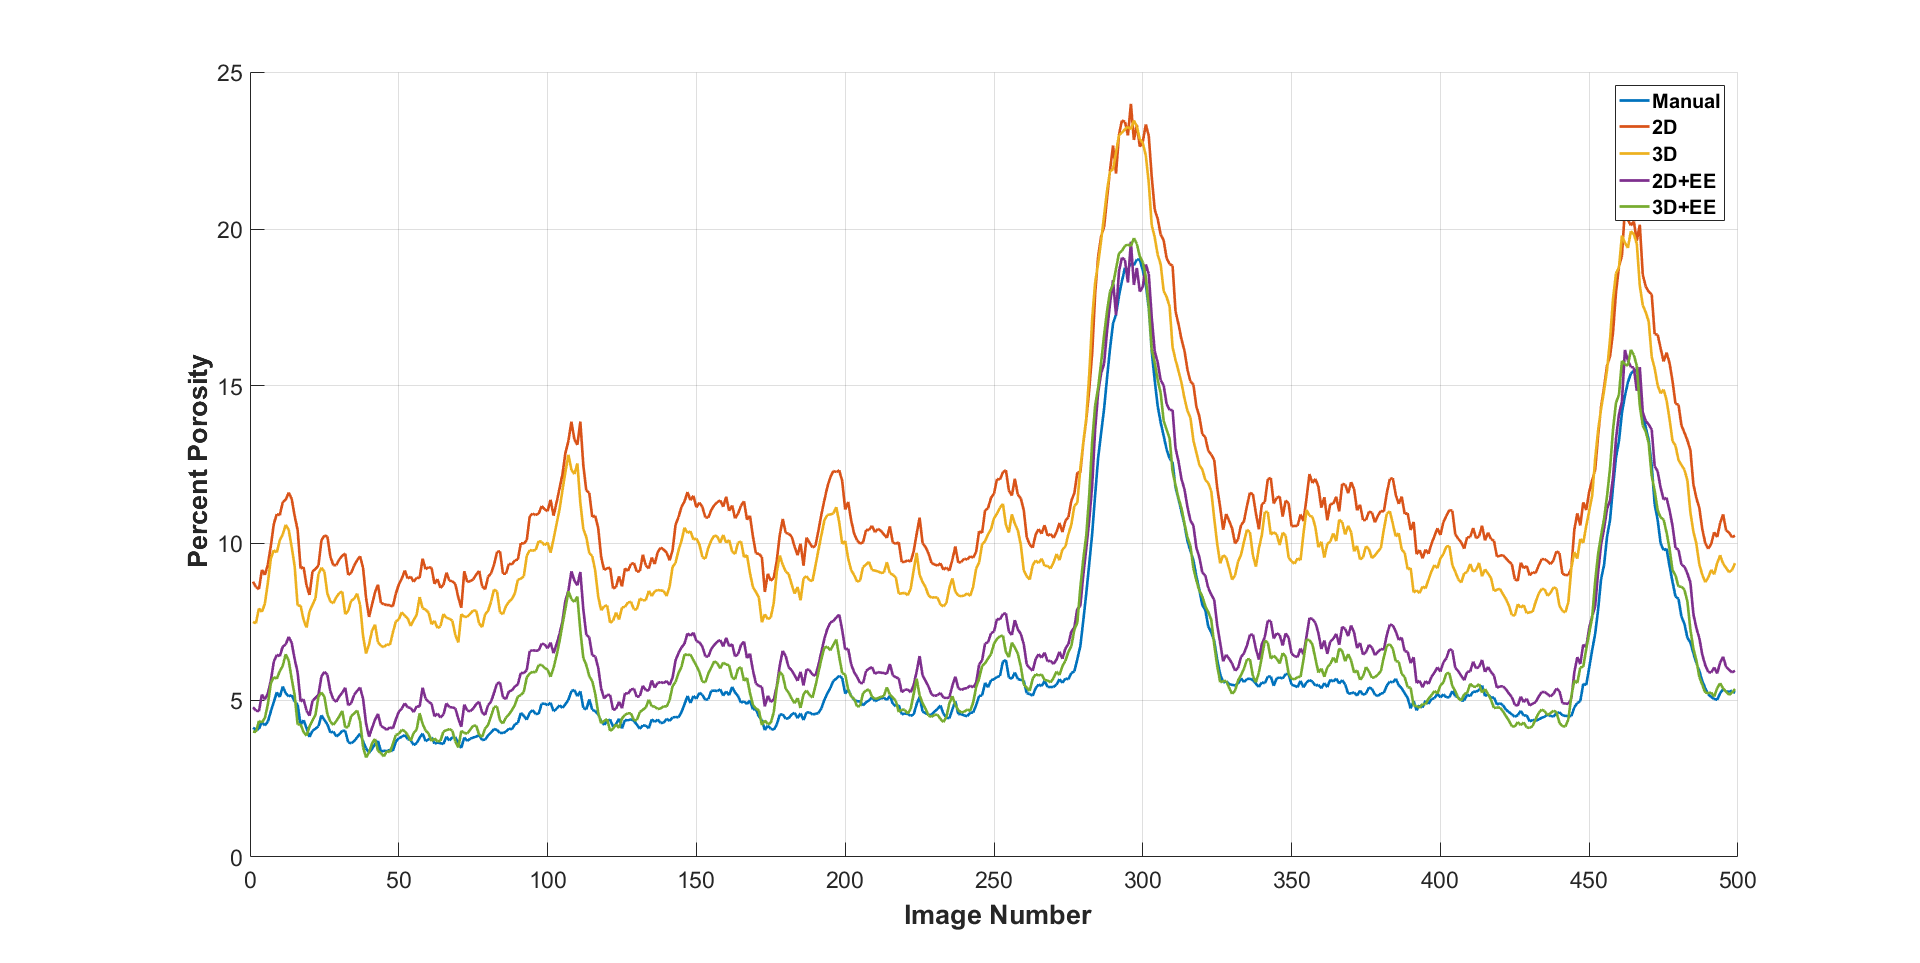
\includegraphics[width=0.55\textwidth]{Porosity.png}
	\caption{Image of percent porosity segmentation for each method on each individual image cross-section.}
	\label{fig:Outy}
\end{figure}

% Table generated by Excel2LaTeX from sheet 'Sheet1'
\begin{table}[htbp]
	\centering
	\caption{Porosity Calculations}
	\begin{tabular}{|l|r|r|r|r|r|}
		\toprule
		Method & \multicolumn{1}{c|}{Manual} & \multicolumn{1}{c|}{2D} & \multicolumn{1}{c|}{3D} & \multicolumn{1}{c|}{2D EE} & \multicolumn{1}{c|}{3D EE} \\
		\midrule
%		Mean  & 0.0599 & 0.1143 & 0.1035 & 0.0715 & 0.0651 \\
		Mean  & 0.060 & 0.114 & 0.104 & 0.072 & 0.065 \\
		\midrule
%		STD   & 0.0316 & 0.0322 & 0.0341 & 0.0311 & 0.0334 \\
		STD   & 0.032 & 0.032 & 0.034 & 0.031 & 0.033 \\
		\bottomrule
	\end{tabular}%
	\label{tab:DataTable}%
\end{table}%
% Table generated by Excel2LaTeX from sheet 'Sheet1'
\begin{table}[htbp]
	\centering
	\caption{One Way ANOVA Results}
	\begin{tabular}{|lrrrrr|}
		\toprule
		\multicolumn{1}{|c}{Source} & \multicolumn{1}{c}{SS} & \multicolumn{1}{c}{DF} & \multicolumn{1}{c}{MS} & \multicolumn{1}{c}{F} & \multicolumn{1}{c|}{$p$} \\
		\midrule
		Group & 1.8878 & 4     & 0.29719 & 281.14 & 0 \\
		Error & 2.63218 & 2490  & 0.00106 &       &  \\
		Total & 3.82096 & 2494  &       &       &  \\
		\bottomrule
	\end{tabular}%
	\label{tab:OneWay}%
\end{table}%

\begin{table}[htbp]
	% table caption is above the table
	\caption{Tukey's HSD multiple Comparisons Results}
	\label{tab:mult}       % Give a unique label
	% For LaTeX tables use
	\begin{tabular}{lll}
		\hline\noalign{\smallskip}
		Method & $p$ \\
		\noalign{\smallskip}\hline\noalign{\smallskip}
		Manual and 2D & 0 \\
		Manual and 3D & 0 \\
		Manual and 2D$+$EE & 0 \\
		Manual and 3D$+$EE & 0.0809 \\
		2D and 3D & 0 \\
		2D and 2D$+$EE & 0 \\
		2D and 3D$+$EE & 0 \\
		3D and 2D$+$EE & 0 \\
		3D and 3D$+$EE & 0 \\
		2D$+$EE and 3D$+$EE & 0.0182 \\
		\noalign{\smallskip}\hline
	\end{tabular}
	\centering
\end{table}

Histograms of percent error calculations in Figure \ref{fig:DiffHist} show that these data are normally distributed. This difference, with respect to the distribution of raw porosity data, can be understood by considering that the percent difference is no longer highly dependent on the image content, but rather on the segmentation method. This allows the percent error to be considered a random variable for further analysis. Mean error and standard deviation are listed in Table \ref{tab:DiffTable}. As expected from the prior analysis, the 3-D WEKA segmentation with Edge Erosion algorithm displayed the lowest error and standard deviation, indicating that it is the desired method of segmentation. Figure \ref{fig:overlay} displays an example of the over prediction in the automatic segmentation and the result of applying the Edge Erosion correction. 

\begin{figure}[h!]
	\centering
	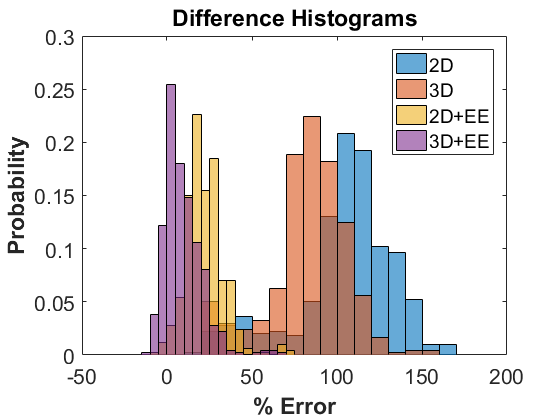
\includegraphics[width=0.5\textwidth]{DifferenceHistograms.png}
	\caption{Histogram of percent error for each of the automatic segmentation methods}
	\label{fig:DiffHist}
\end{figure}
% Table generated by Excel2LaTeX from sheet 'Sheet2'
\begin{table}[htbp]
	\centering
	\caption{Percent Error Calculations}
	\begin{tabular}{|l|r|r|r|r|}
		\toprule
		Meathod & \multicolumn{1}{c|}{2D} & \multicolumn{1}{c|}{3D} & \multicolumn{1}{c|}{2D EE} & \multicolumn{1}{c|}{3D EE} \\
		\midrule
		Mean  & 104.21 & 82.56 & 22.33 & 9.22 \\
		\midrule
		STD   & 29.05 & 23.18 & 11.21 & 11.00 \\
		\bottomrule
	\end{tabular}%
	\label{tab:DiffTable}%
\end{table}%


\begin{figure}[h!]
	\centering
	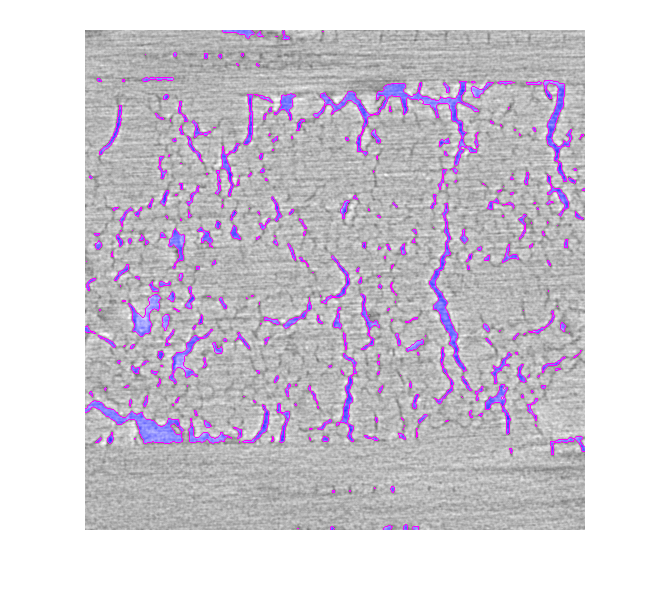
\includegraphics[width=0.5\textwidth]{overlay.png}
	\caption{Image of the material microstructure overlaid with porosity segmentation. Red corresponds to the over-prediction of automatic segmentation when compared to the manual method, and purple corresponds to porosity.}
	\label{fig:overlay}
\end{figure}

Finally, the factorial analysis resulted in the following linear regression equation:
\begin{multline}
Percent Error= 54.5790 - 8.6906 X_A \\
- 38.8059 X_B + 2.1367 X_A X_B
\end{multline}
where $X_A$ and $X_B$ represent the coded variables for analysis dimension and edge erosion respectively. A response surface is plotted in Figure \ref{fig:Surf}. This analysis shows that the pixel erosion contributes more to segmentation accuracy in contrast to the dimensionality of the WEKA segmentation algorithm. This result could be useful for applying these techniques to larger data sets where computer memory and computational time becomes a limiting factor for 3-D methods. The results of the two-way ANOVA in Table \ref{tab:TwoWay} show that all effects measured in the factorial analysis were statistically significant. 

\begin{figure}[h!]
	\centering
	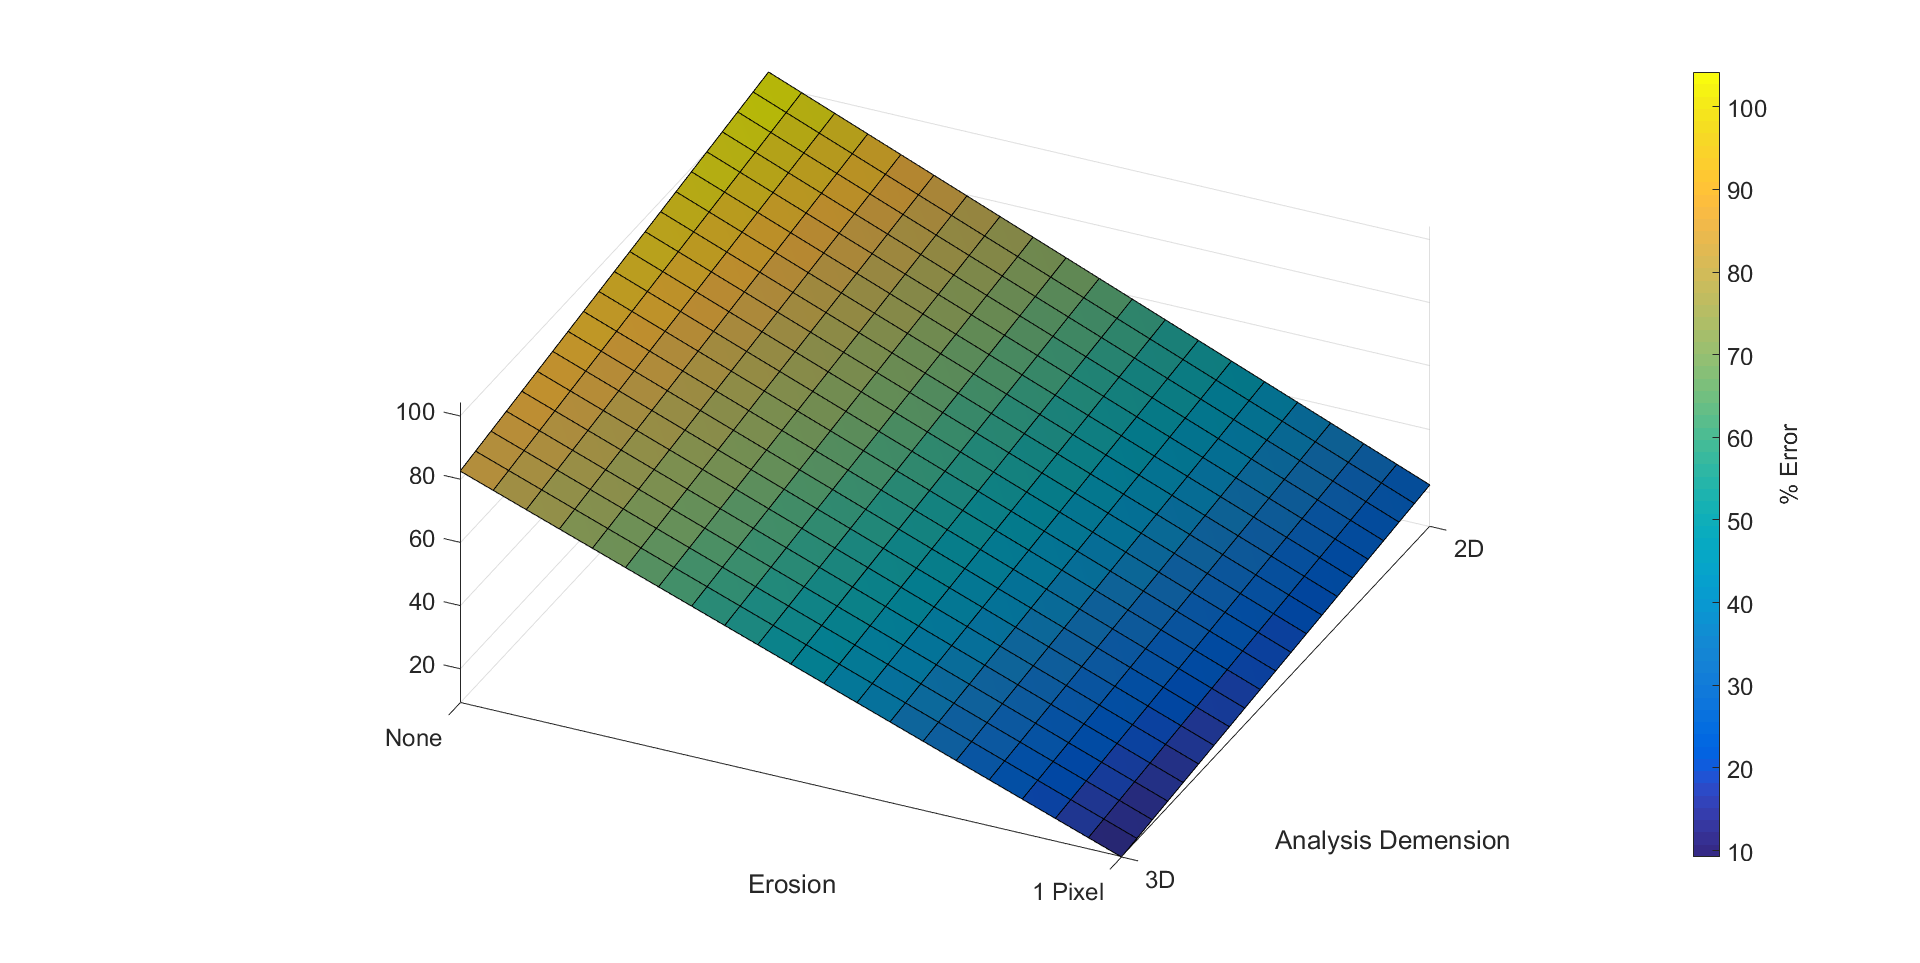
\includegraphics[width=0.5\textwidth]{ResponseSurface.png}
	\caption{Response surface model for two different algorithm features}
	\label{fig:Surf}
\end{figure}



% Table generated by Excel2LaTeX from sheet 'Sheet2'
\begin{table}[htbp]
	\centering
	\caption{Two Way ANOVA for factorial analysis}
	\begin{tabular}{|lrrrrr|}
		\toprule
		\multicolumn{1}{|c}{Factor} & \multicolumn{1}{c}{SS} & \multicolumn{1}{c}{DF} & \multicolumn{1}{c}{MS} & \multicolumn{1}{c}{F} & \multicolumn{1}{c|}{$p$ } \\
		\midrule
		Dimensionality & 15.1 & 1     & 15.08 & 370.4 & 0 \\
		Edge Erosion & 300.6 & 1     & 300.58 & 7386.0 & 0 \\
		Interaction & 0.91 & 1     & 0.911 & 22.39 & 0 \\
		Error & 81.1 & 1992  & 0.041 &       &  \\
		Total & 397.6 & 1995  &       &       &  \\
		\bottomrule
	\end{tabular}%
	\label{tab:TwoWay}%
\end{table}%


\subsection{Error and Uncertainties} 
Image analysis and segmentation are inherently prone to error. Digital imaging captures light reflected by, or transmitted through a continuous media and records discretized values of light intensity. If image discretization does not exactly match boundaries within the image subject, distortion and blurring of edges will occur. Image noise further confounds the distinction of image contents. The human visual system is effective at interpreting image contents, but interpretation can vary widely from person to person.\\
The analysis here used manually segmented images as a ``ground truth" for comparison between methods, but the chosen segmentation could have easily contained slight variations if another person had conducted the segmentation. The attractiveness of automatic segmentation lies in both its speed \textit{and} repeatability. Until imaging tools are capable of producing sharp enough images that there are no questionable ``edge cases" for segmentation, there will always remain some small unquantifiable uncertainty in segmentation methods. However, by using the same algorithm across data sets for the purposes of comparison, this uncertainty can be ignored because it is present in all data sets.\\
Furthermore, potential error can be attributed to the assumptions required for ANOVA. It was shown in Figure \ref{fig:Boxy} that the distribution in percent porosity calculation for individual image cross-sections did not meet a normal distribution. The conditions for independence and homoscedasticity were satisfied. In Figure \ref{fig:Outy}, outliers were present for a small range of images, and were consistent for all automatic segmentation methods presented. The removal of these images from the data set could improve the overall confidence in the results.


\section{Conclusion and Future Directions} 

In summary, this work demonstrates the ability of an automatic segmentation algorithm to produce results with no statistically significant differences from a manually segmented $\mu$CT image data set. In all cases, the null hypothesis was rejected with the exception of the 3-D WEKA and Edge Erosion method ($p$=0.081), indicating that the algorithm produced acceptable image segmentation. Average error for this algorithm of less than 10\% was achieved. It is possible that this value can be further reduced by additional training to the underlying machine learning architecture. Pixel erosion was shown to be an effective method to compensate for the architecture's tendency to over-predict image porosity.\\
Future work will include additional testing of the algorithms presented here on full-volume data sets. The current work was only performed on a small sub-volume of the entire image data collected at this particular stage in the manufacturing process. Additionally, performing this study upon several image stacks across the entire manufacturing process will provide more insight on how the proposed automatic segmentation method will perform across multiple data sets. Lastly, no analysis was performed on the effect of image pre-processing. This step in the automatic segmentation methods was implemented in order to reduce the signal to noise ratio while preserving image fidelity. Further studies of additional image stack pre-processing methods could further improve the accuracy of automatic segmentation.

%\bibliographystyle{ieeetr}
\bibliography{DoE_References}

\end{document}